\chapter{Introduction}

\section{Motivation}

A large number of machine learning applications rely on a vast amount of data from the real world to infer useful relations. However, obtaining these data is not always a viable option. The problems with obtaining data are multiple -- i.e. human labor costs for labeling, hardware wear and situations impossible to create in real world (such as crashing). Luckily, computer graphics started to become more and more realistic in recent years~\cite{matrix}, and it is now possible to capture image and depth data from computer games. These data have one significant advantage -- it can simulate almost any scenario such as crashing, unusual environment, etc., as long as it is possible within the game.

Although the data captured from the modern computer games look almost realistic, it suffers from many problems to be readily usable by machine learning applications. The most significant drawback is the fact, that they look {\em too} perfect -- real-world sensors often measure data with noise or fail altogether.

Our goal in this thesis is to find such a mapping between the in-game data and the real world data to be able to transform the in-game data to look as realistically as possible. Since we do not have a one-to-one correspondences between these data, it is necessary to apply methods of {\em unsupervised} learning. Recently, a new method suitable for unsupervised generative learning called CycleGAN~\cite{cyclegan} emerged and it is based on Generative Adversarial Networks (GANs)~\cite{origgan}. This method was shown to work on various unpaired image datasets, however, as far as we know this is the first work which is trying to apply it on LiDAR measurements. For better understanding of the work see schema of the algorithm in the figure \ref{schema}.

\begin{figure}
\centering
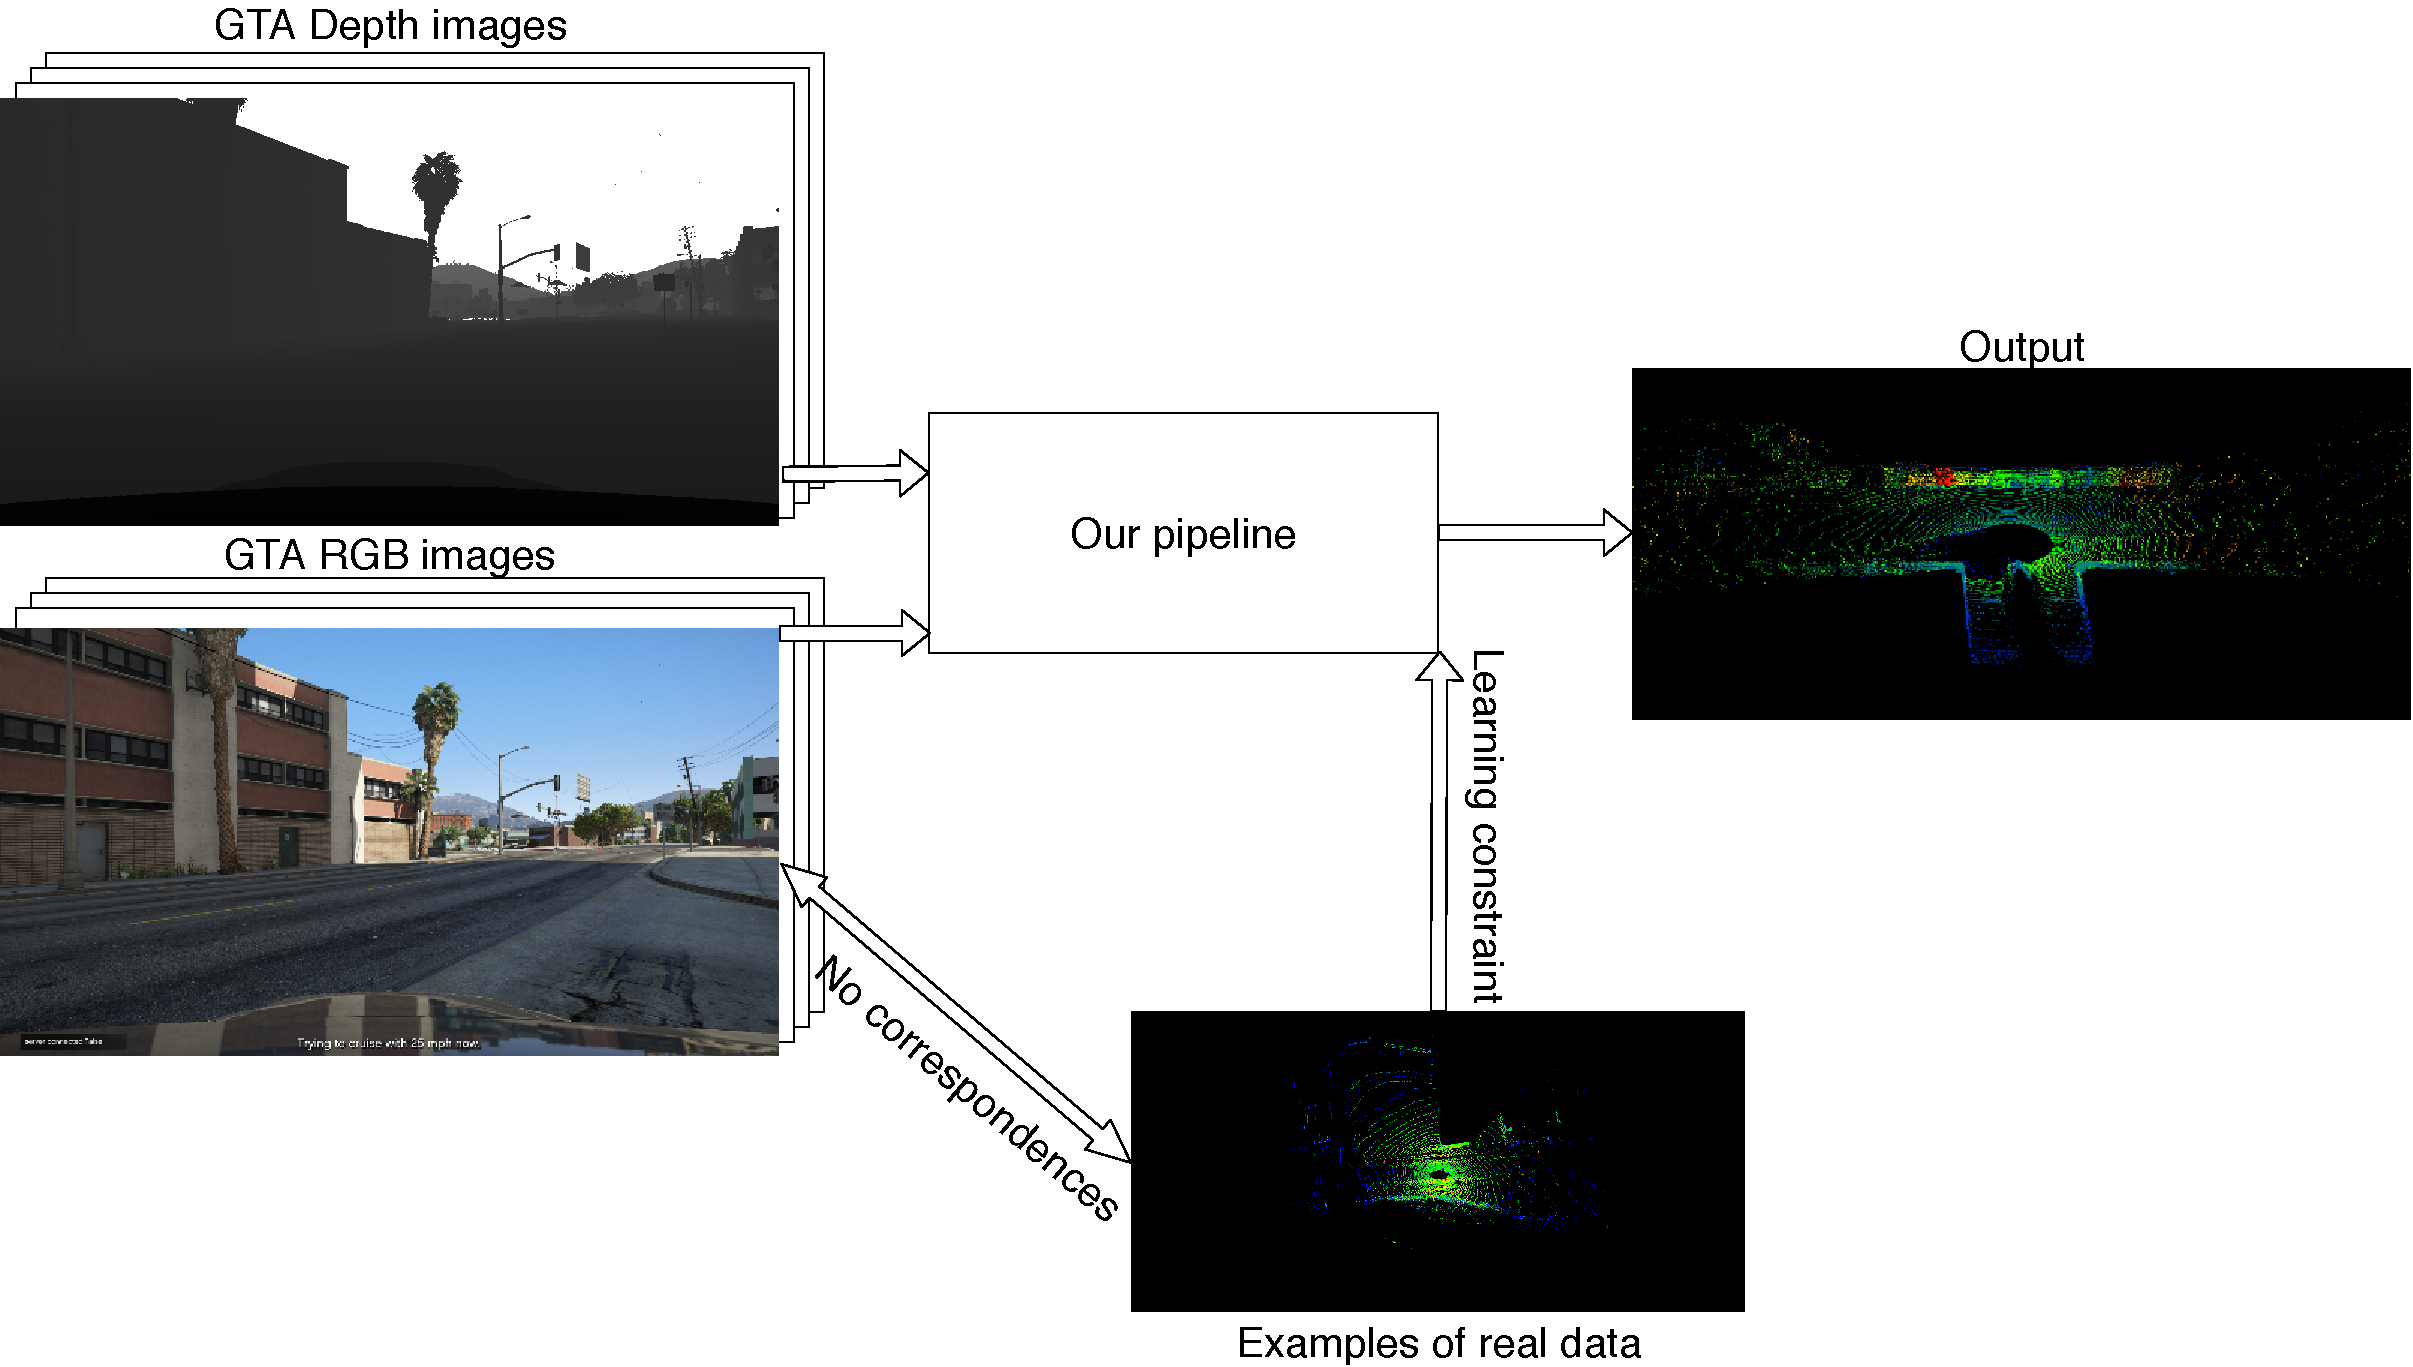
\includegraphics[keepaspectratio, width=0.98\textwidth]{img/algorithm.pdf}
\caption{Schema of the algorithm}
\label{schema}
\end{figure}

\section{Contribution}
Main contribution of this thesis was to show that CycleGAN and by extension generative modeling applied to LiDAR sensors is feasible. The resulting generators added reasonable amount of noise to the data while being able to distinguish between different objects in the scene. It is therefore reasonable to assume that the generators are able to learn different amount of noise induced by different surfaces in the real world.

\section{Thesis structure}
In this first chapter, we set up motivation and reasoning for this work and also briefly summarize contribution of this thesis. The next chapter is an overview of related theoretical work. The first section of said chapter briefly summarizes recent work in the field, while the next section explores more deeply neural networks used in this thesis. The last section of this chapter describes operation of LiDAR which we are trying to simulate in chapter \ref{experiments}.

Chapter \ref{dataset} is dedicated to the used datasets. In this chapter, we summarize key characteristics of the datasets and how they were obtained.

Chapter \ref{programs} describes all the programs written for the purpose of this thesis and shows their functionality. This chapter can also serve as a user guide for the programs.

Chapter \ref{experiments} describes the performed experiments. We also describe all the drawbacks we encountered during the experiments. The chapter ends with a showcase of results.

In the last chapter, we analyze all the results and discuss the achieved contributions of this thesis, followed by plans for the future work and conclusion.
